\subsection{Training the CNN-LSTM Agent Using PPO2}

\begin{wrapfigure}{r}{0.5\textwidth}
\vspace{-1.0cm}
  \begin{center}
    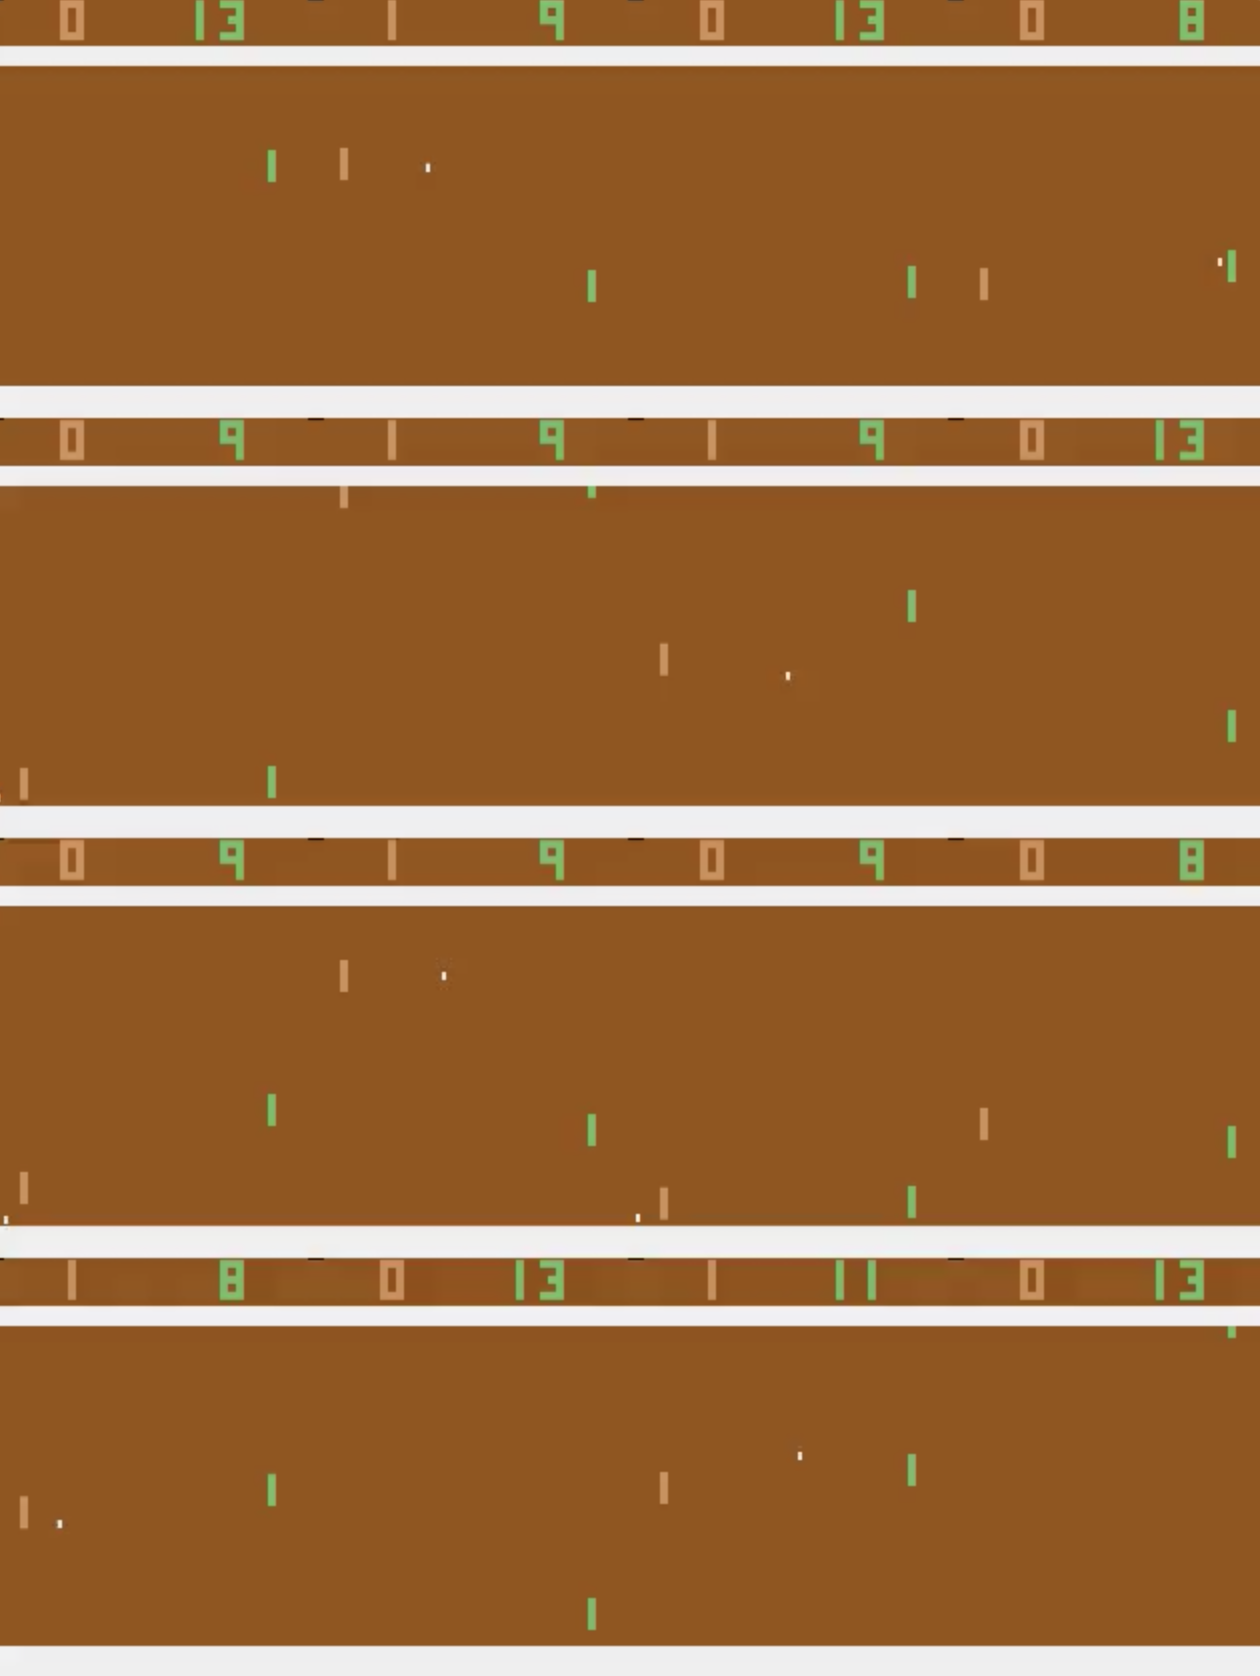
\includegraphics[width=0.5\textwidth]{Figures/multi_env_cnn-lstm_agent.png}
  \end{center}
  \caption{A figure showing the vectorized environment the PPO2 agent trained in. As PPO2 works with rollouts of the policy and not active interaction, rollouts are easily parallelized and greatly aid training speed. Training in a parallelized environment took many hours fewer than in scalar environment.}
  \label{fig: multi_env_cnn-lstm_agent}
  \vspace{0.4cm}
\end{wrapfigure}

In Tables \ref{t: ppo2_arch} and \ref{t: ppo2_hparams} we defined the CNN-LSTM agent and the PPO2 hyperparameters used to train the agent. Figure \ref{fig: ppo2_main_loss} shows the "main" policy gradient loss evolution with environment step, while Figures \ref{fig: ppo2_entropy_loss_term} - \ref{fig: ppo2_value_function_loss} show how the individual components of this overall loss evolve.

The agents episodic reward is shown in Figure \ref{fig: ppo2_reward}, where we can see that at the end of the 7M training steps, the agent is consistently getting the maximum reward for the environment. The vectorized training environment for the CNN-LSTM can be seen in Figure \ref{fig: multi_env_cnn-lstm_agent}.

\begin{figure}
    \centering
    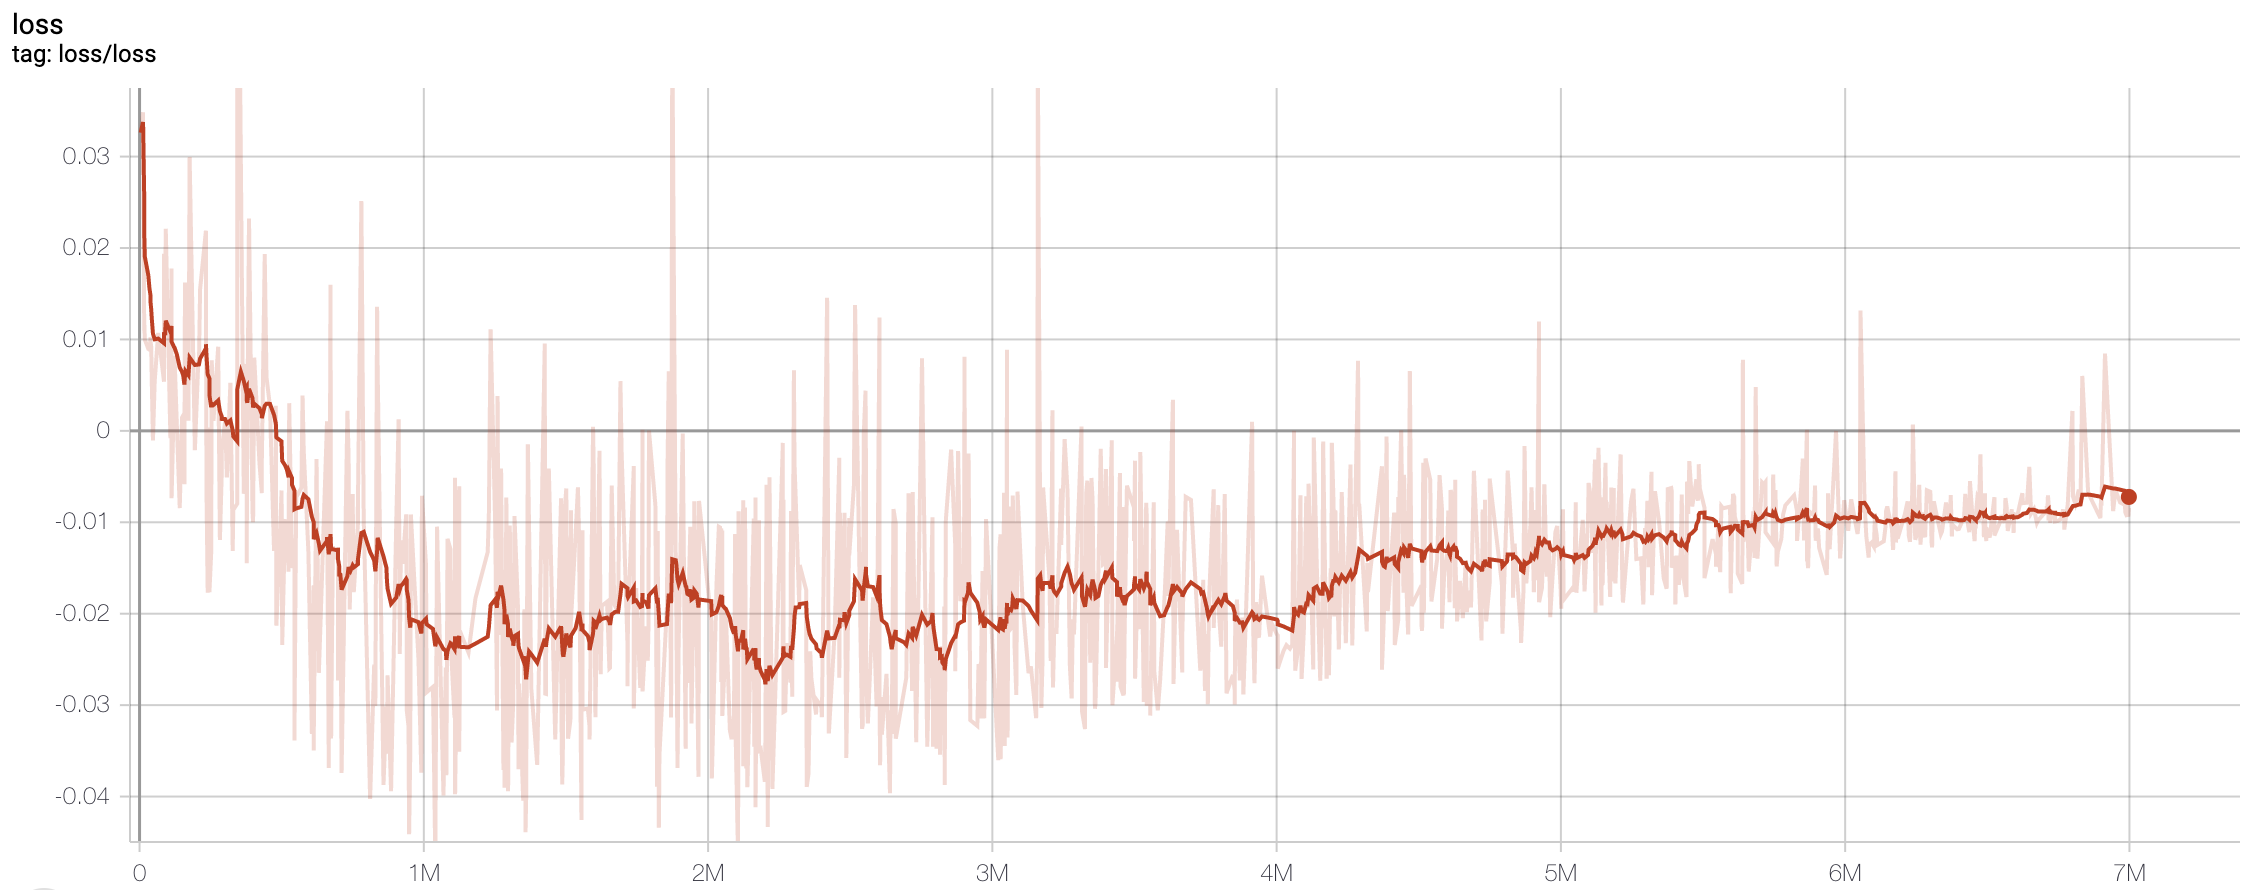
\includegraphics[width=\textwidth]{Figures/ppo2_main_loss.png}
    \caption{The full PPO2 loss term (objective function) per environmental step, $L_{t}^{C L I P+V F+S}(\theta)$, of the overall policy gradient loss used by PPO2, with the final network and training settings. We can see that just as with most RL algorithms, even with extremely large numbers of samples the loss does not go to zero, especially as the objective function for PPO2 is only approximately optimized during training \cite{PPO2}.}
    \label{fig: ppo2_main_loss}
\end{figure}

\begin{figure}
    \centering
    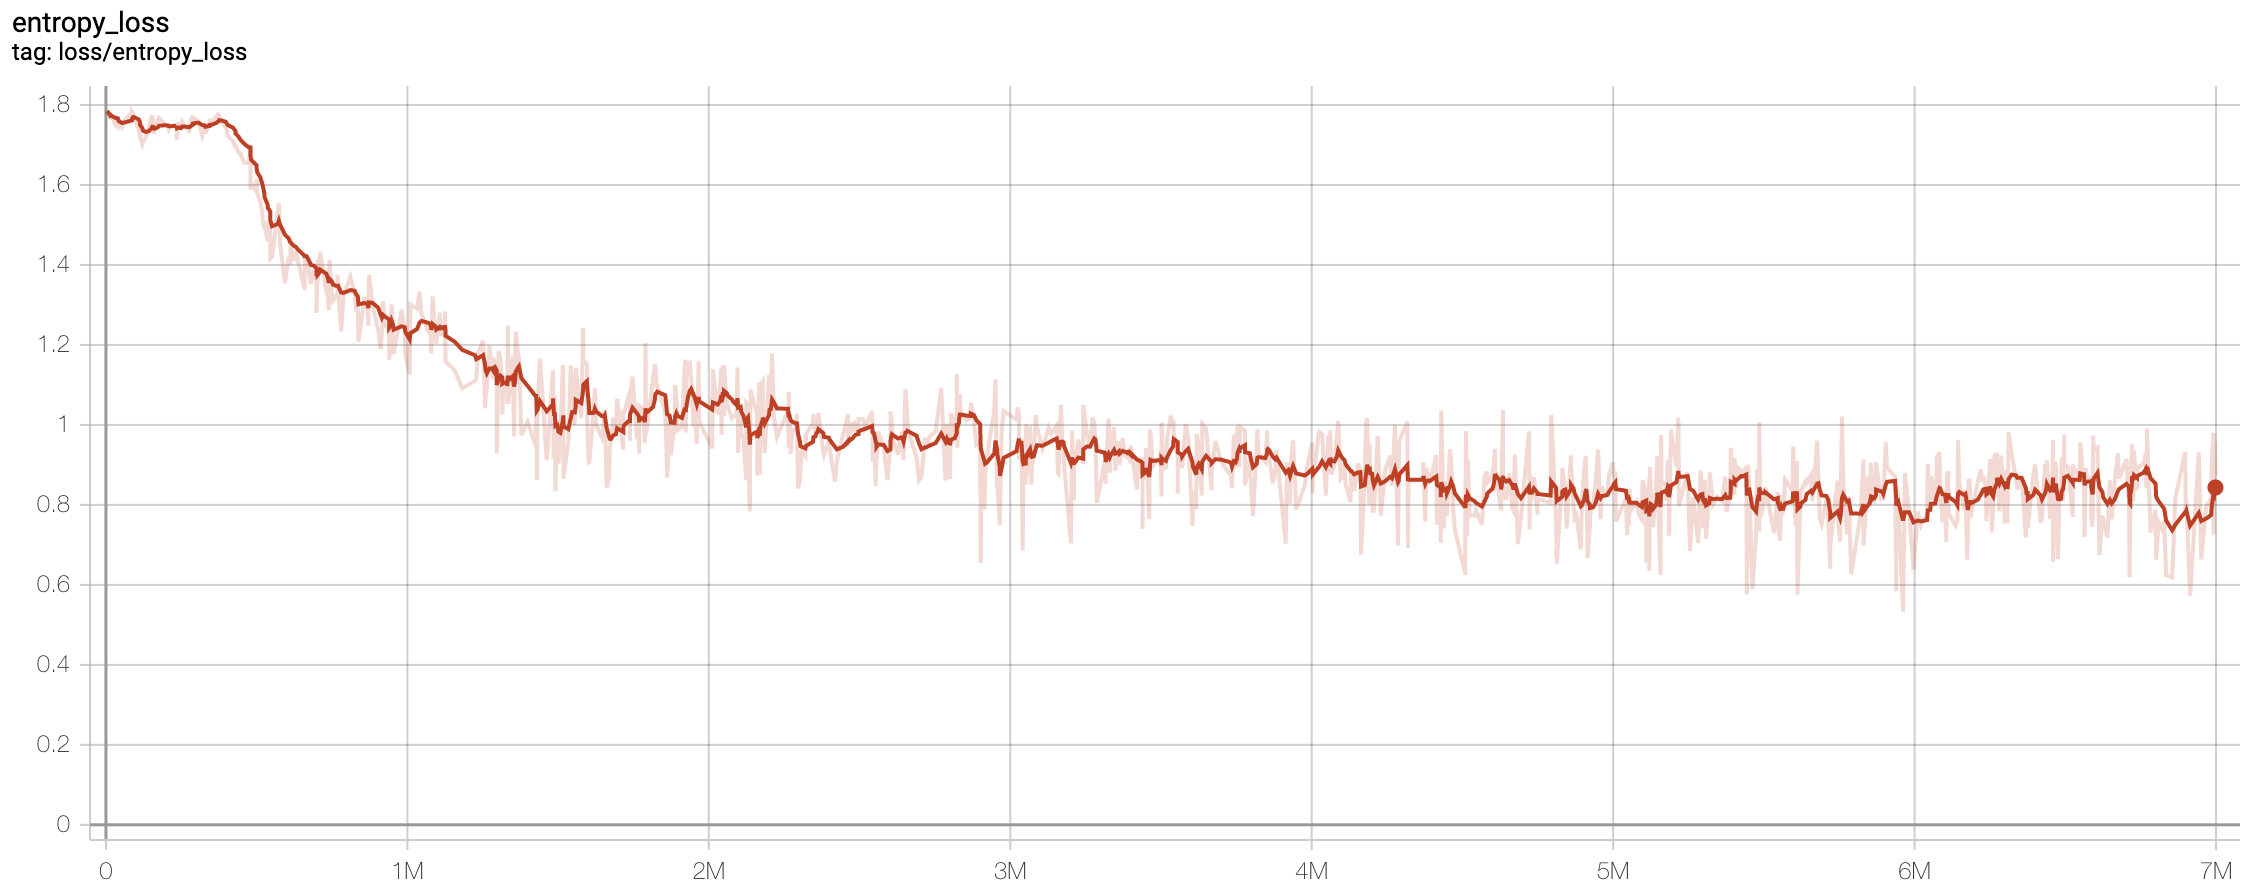
\includegraphics[width=\textwidth]{Figures/ppo2_entropy_loss_term.png}
    \caption{The entropy term per environment step, $S\left[\pi_{\theta}\right]$, of the overall policy gradient loss used by PPO2, with the final network and training settings. Notice that the entropy, which should be maximized as an objective in PPO2 \cite{PPO2}, actually decreases with each episode. I suspect the agent began trading off policy entropy for perhaps better surrogate objective ($L_{t}^{C L I P}(\theta)$).}
    \label{fig: ppo2_entropy_loss_term}
\end{figure}

\begin{figure}
    \centering
    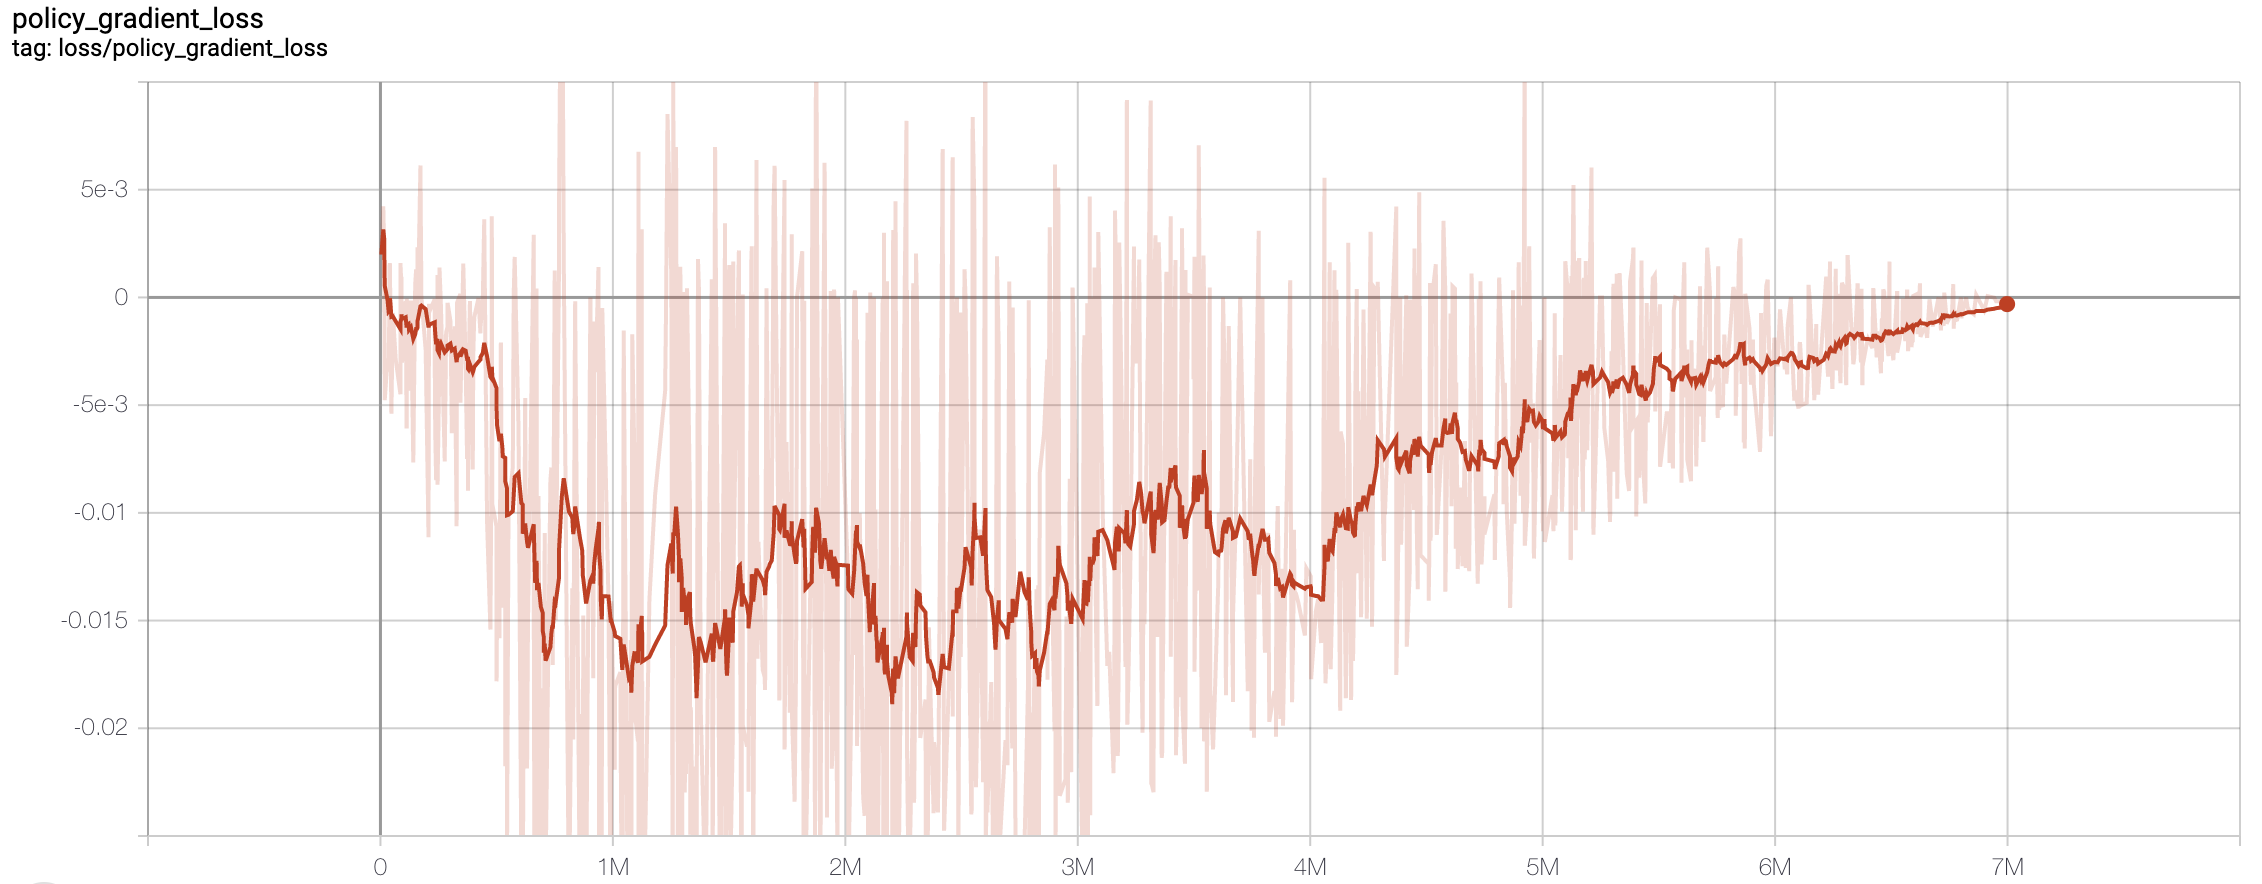
\includegraphics[width=\textwidth]{Figures/ppo2_surrogate_loss.png}
    \caption{The surrogate PPO2 loss term (the objective function based on a trust region \cite{PPO2}) per environmental step, $L_{t}^{C L I P+V F+S}(\theta)$, of the overall policy gradient loss used by PPO2, with the final network and training settings. The agent needed all 7M steps to reduce this loss term, here based on the "probability ratio clipping" surrogate loss \cite{PPO2}, to 0 which it impressively did.}
    \label{fig: ppo2_surrogate_loss}
\end{figure}

\begin{figure}
    \centering
    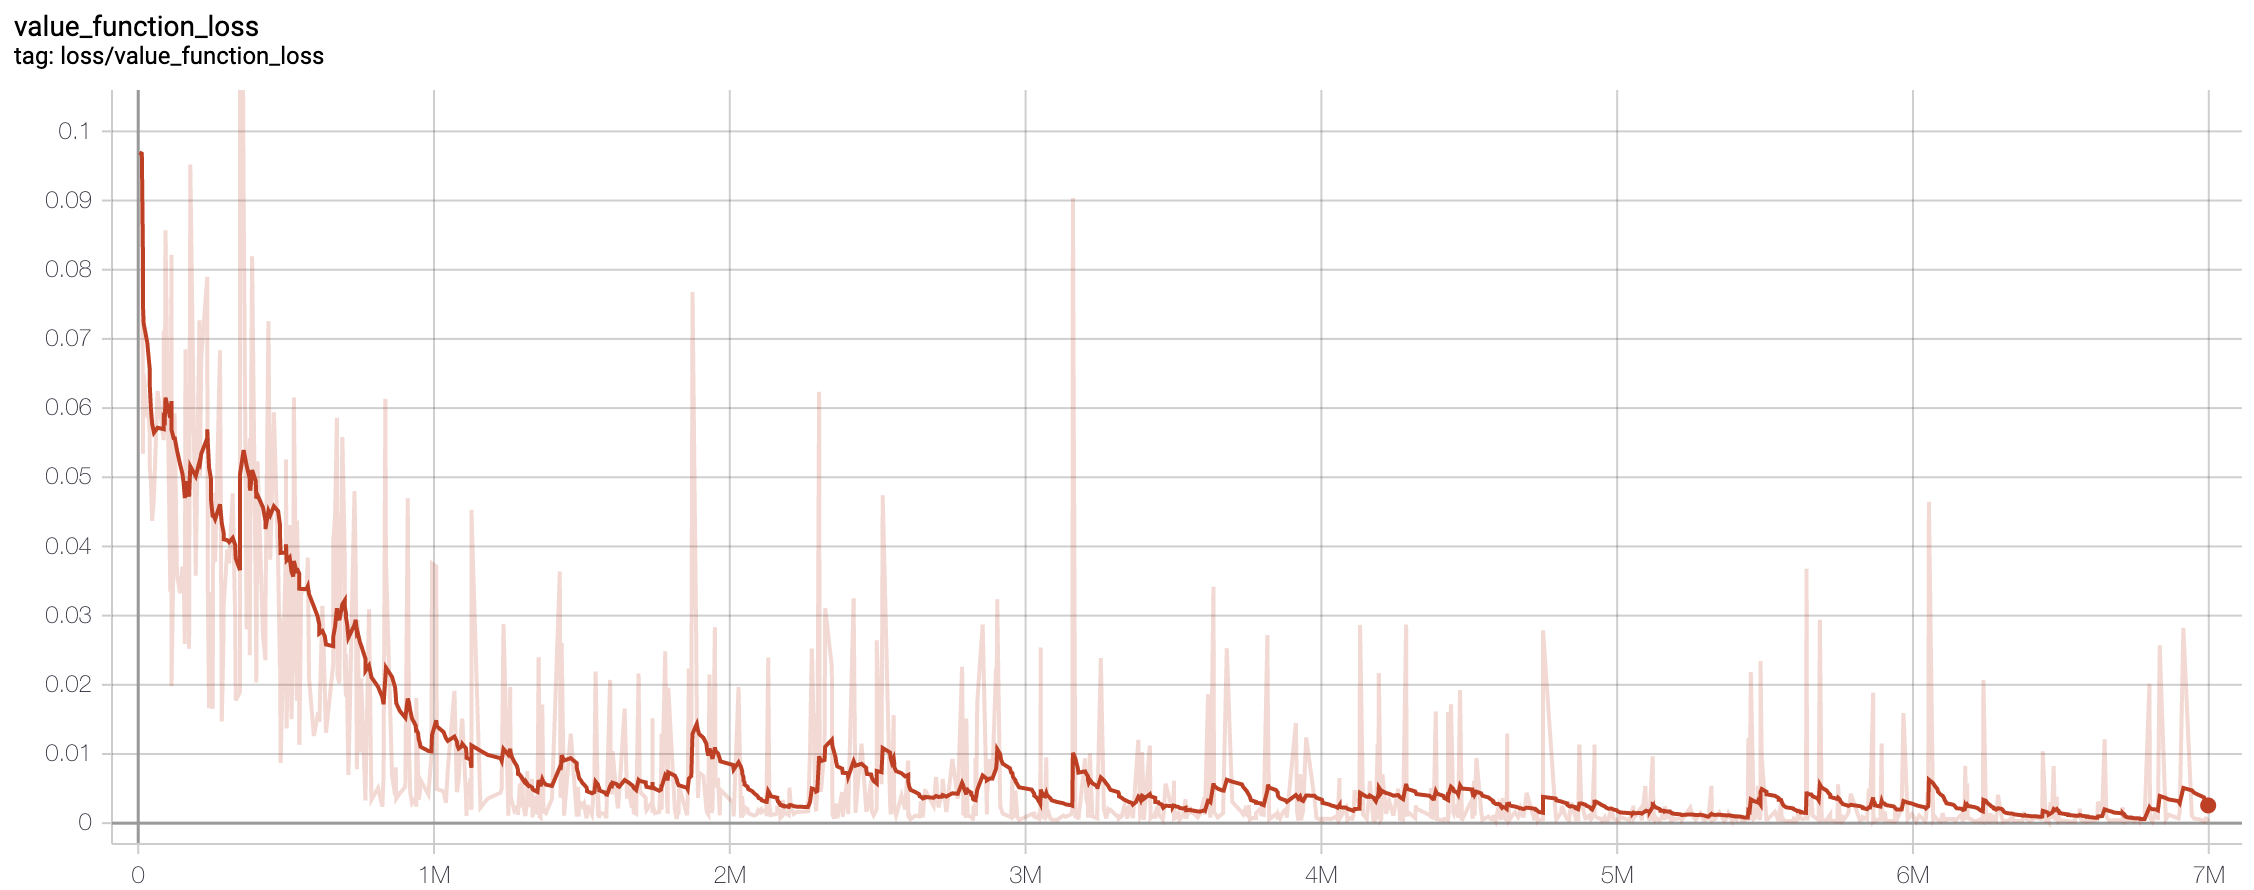
\includegraphics[width=\textwidth]{Figures/ppo2_value_function_loss.png}
    \caption{The value PPO2 loss term per environmental step, $L_{t}^{V F}(\theta)$, of the overall policy gradient loss used by PPO2, with the final network and training settings. This loss, which is based on the actor-critic architecture of the output layers, was nicely driven to 0 by the end of the training process.}
    \label{fig: ppo2_value_function_loss}
\end{figure}

\begin{figure}
    \centering
    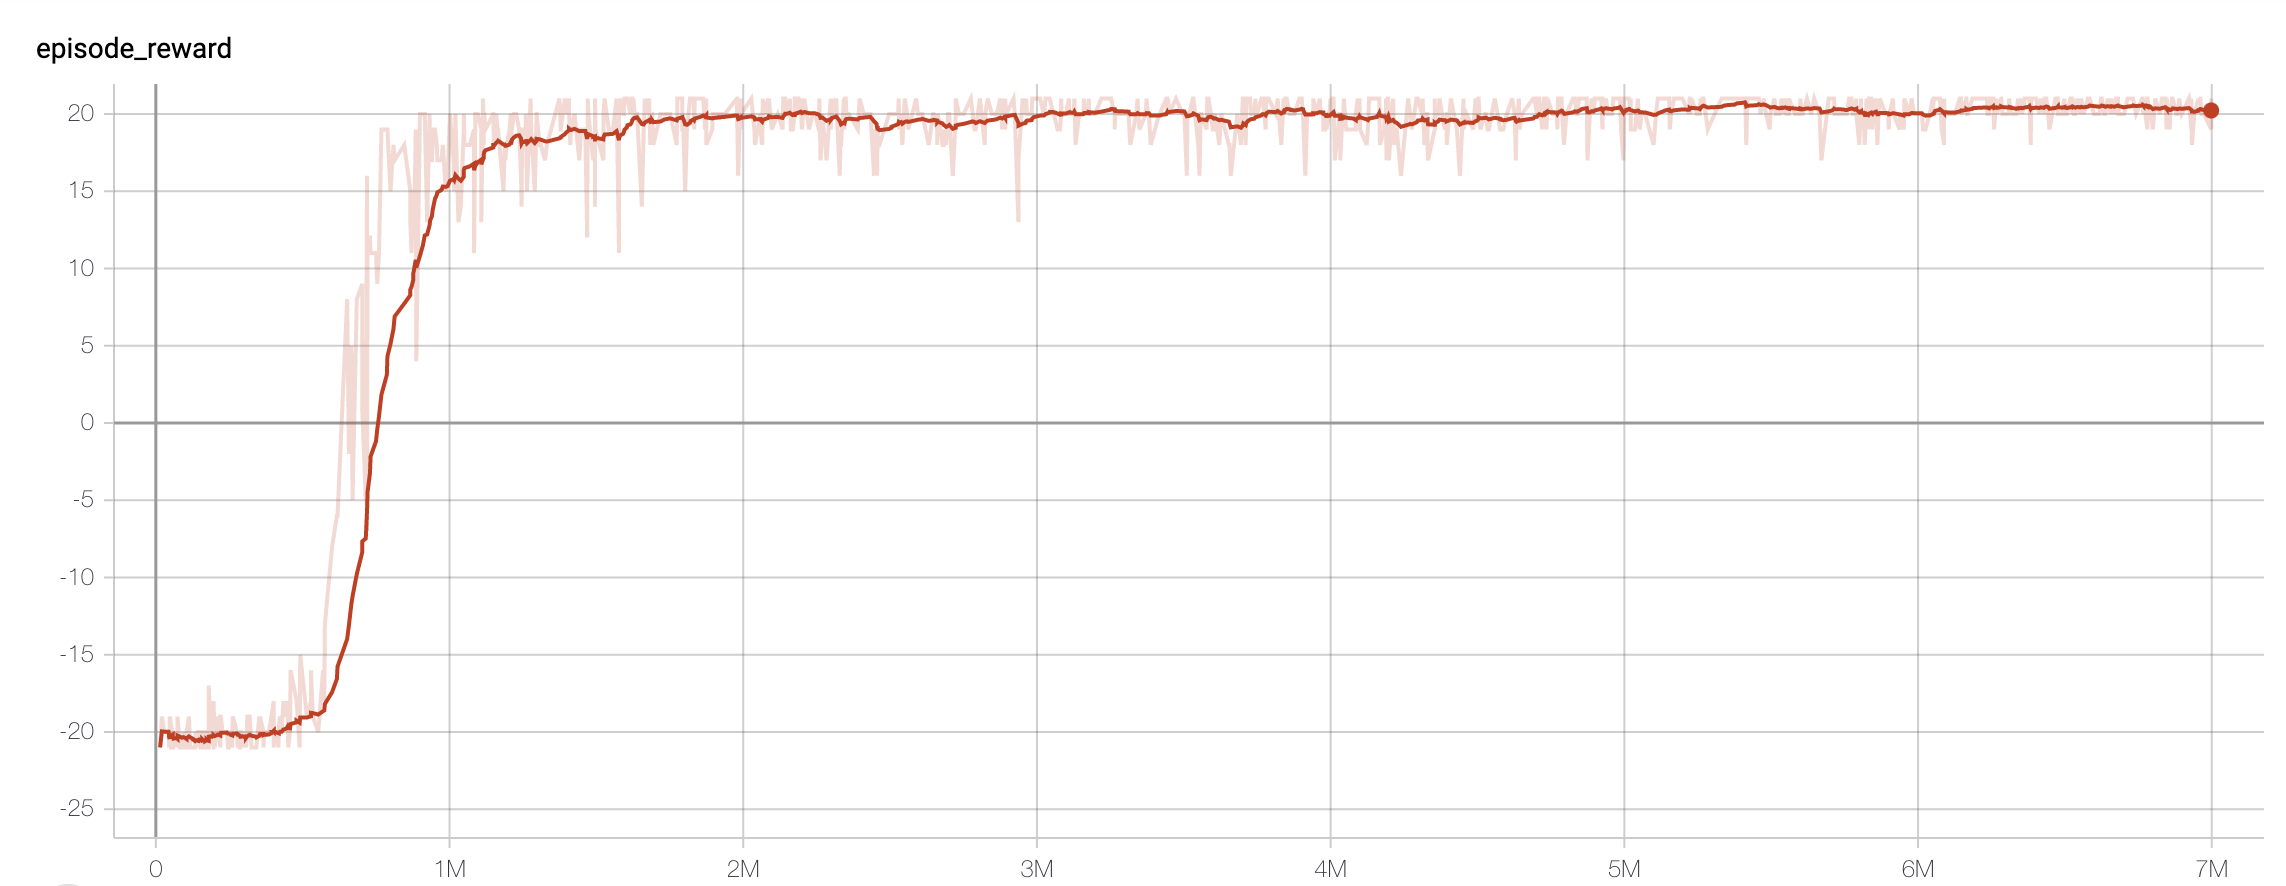
\includegraphics[width=\textwidth]{Figures/ppo2_reward.png}
    \caption{The PPO2 agent's episodic reward. While it may appear that we could have finished training much earlier than at 7M steps, based on the loss curves shown in the other plots, the agent was still stabilizing and internally improving. Qualitatively, my experience was that the agent needed significant time after first reaching the maximum episodic reward (21) to be reliable and smooth when visualized. A good example of how reward signals are rarely capable of encoding the fully desired task specification.}
    \label{fig: ppo2_reward}
\end{figure}

%%%%%%%%%%%%%%%%%%%%%%%%%%%%%%%%%%%%%%%%%%%%%%%%%%%%%%
%%%%%%%%%%%%%%%%%%%%%%%%%%%%%%%%%%%%%%%%%%%%%%%%%%%%%%
%%%%%%%%%%%%%%%%%%%%%%%%%%%%%%%%%%%%%%%%%%%%%%%%%%%%%%
\subsection{Training the Quantized Bottleneck Networks}

The observation QBN was trained using the parameters found in Tables \ref{t: obs_qbn_arch} \& \ref{t: obs_qbn_hparams}. We can see the evolution of the reconstruction MSE loss on the sampled observation features from the CNN of the CNN-LSTM policy with training epoch in Figure \ref{fig: obs_qbn_loss}.

\begin{figure}
    \centering
    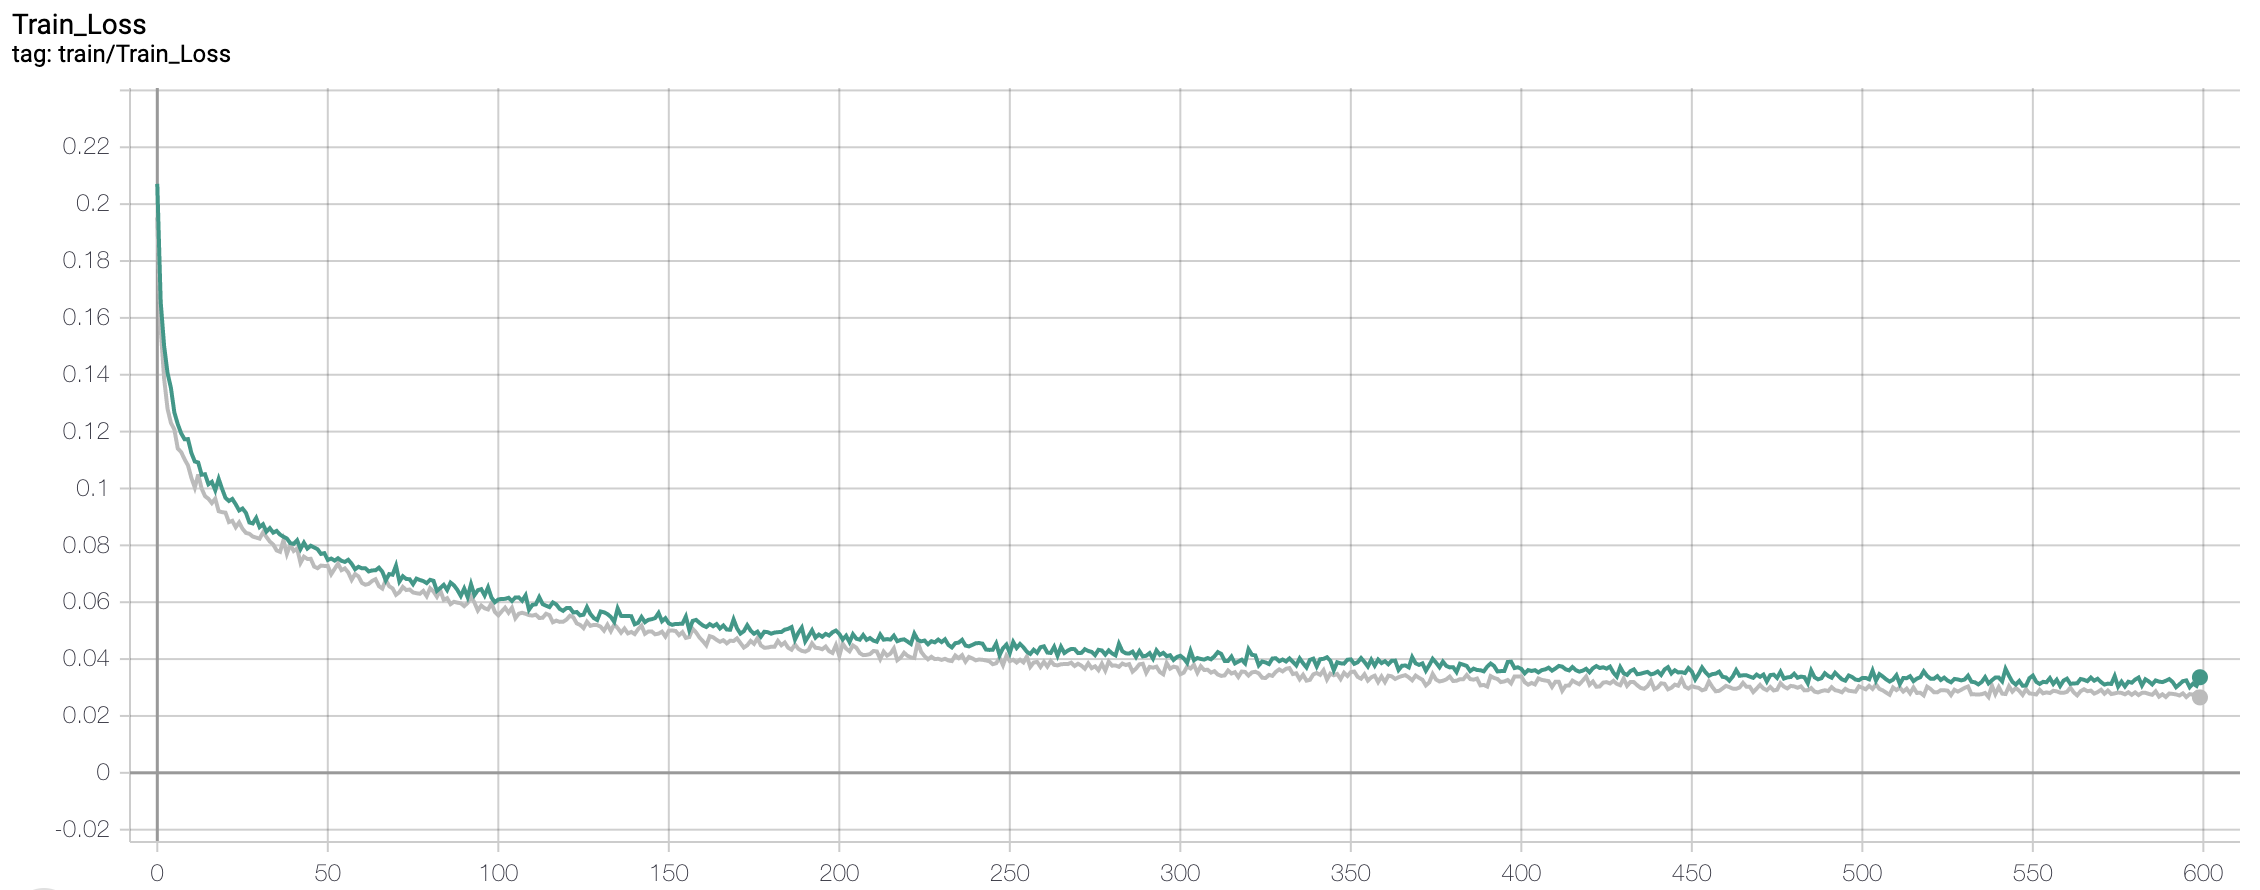
\includegraphics[width=\textwidth]{Figures/hid_state_qbn_loss.PNG}
    \caption{The training and test losses vs. epoch for the final QBN model used to quantize and compress the hidden state output of the LSTM module of the learned Atari agent's policy.}
    \label{fig: hid_state_qbn_loss}
\end{figure}

The hidden state QBN was trained using the parameters found in Tables \ref{t: hid_state_qbn_arch} \& \ref{t: hid_state_qbn_hparams}. We can see the evolution of the reconstruction MSE loss on the sampled hidden states of the LSTM module in the CNN-LSTM policy with training epoch in Figure \ref{fig: hid_state_qbn_loss}.

\begin{figure}
    \centering
    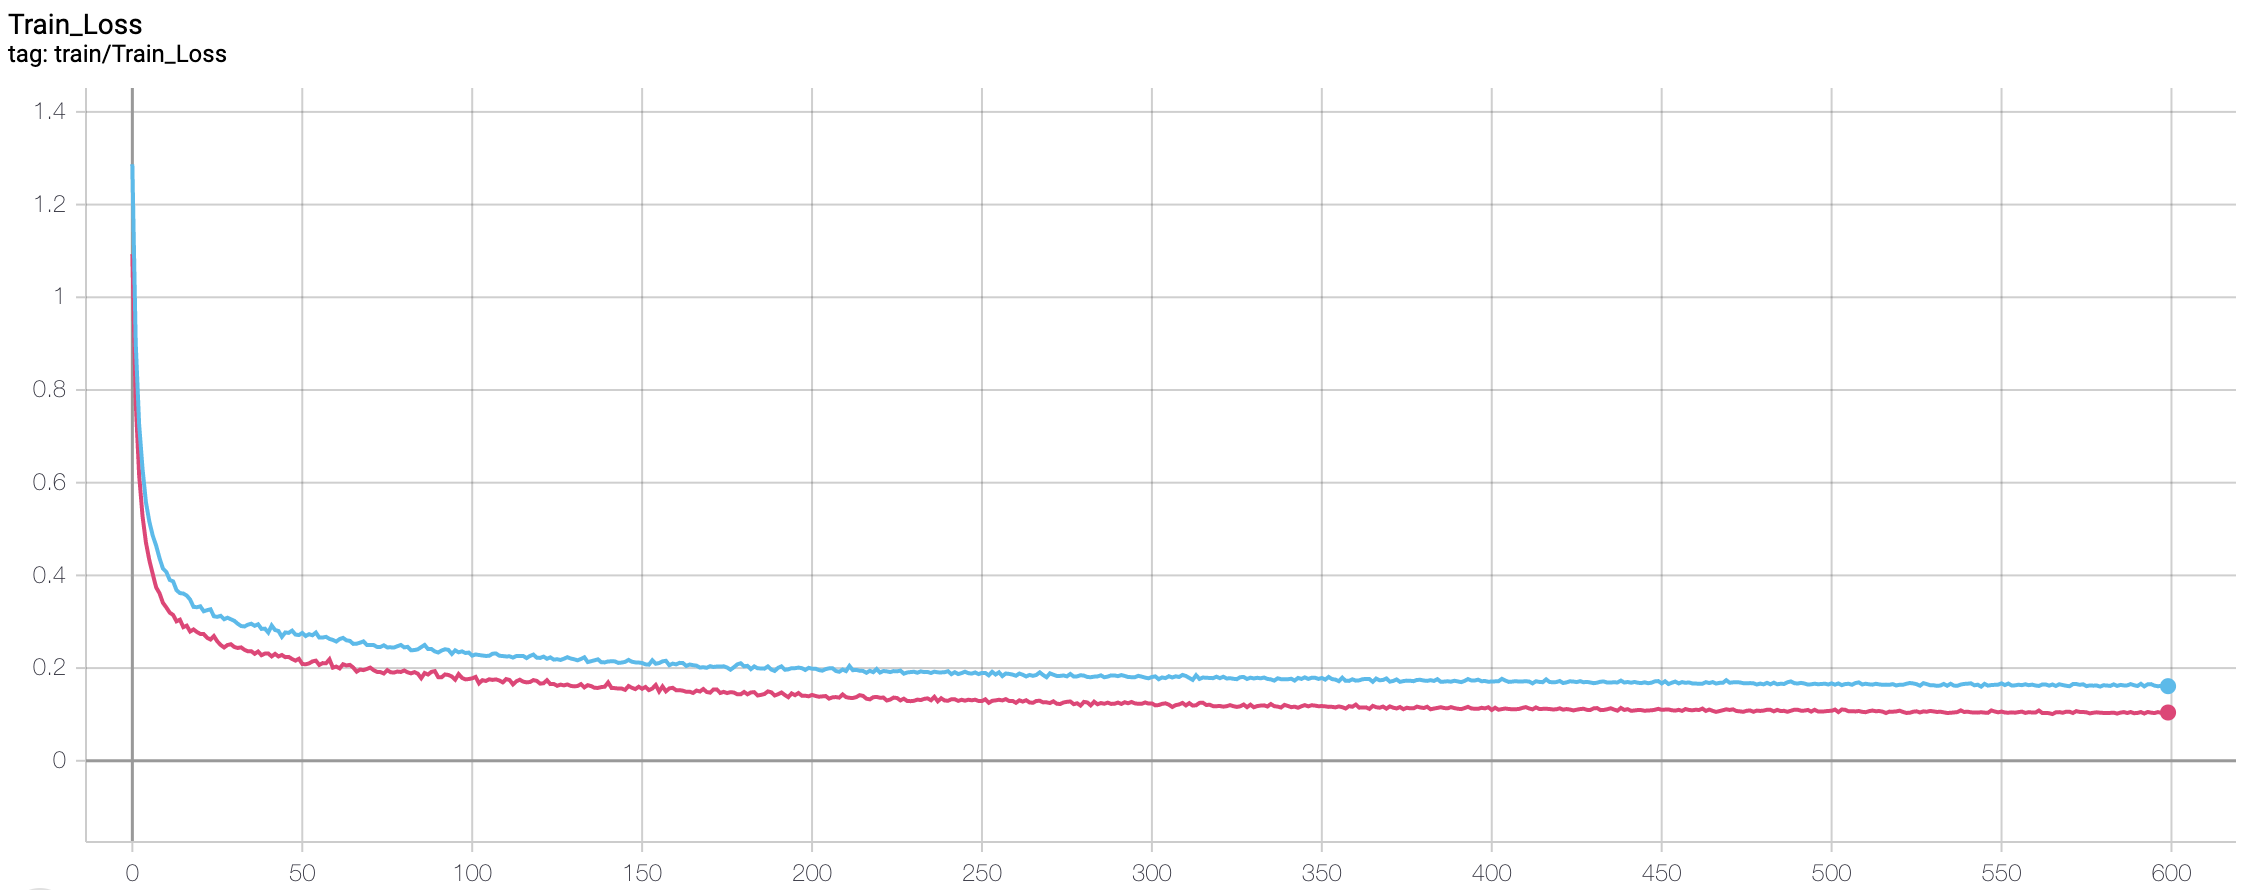
\includegraphics[width=\textwidth]{Figures/obs_qbn_loss.png}
    \caption{The training and test losses vs. epoch for the final QBN model used to quantize and compress the flattened convolutional feature output of the CNN feature extractor module of the learned Atari agent's policy. I had a lot of trouble getting this the same QBN architecture used in the Koul et. al. paper \cite{Koul2019} to converge to a near-zero loss, but I was also using the original atari CNN architecture \cite{nature_q_learning} instead of the that in the Koul paper - a more complex CNN than the one use by Koul et. al.}
    \label{fig: obs_qbn_loss}
\end{figure}


%%%%%%%%%%%%%%%%%%%%%%%%%%%%%%%%%%%%%%%%%%%%%%%%%%%%%%
%%%%%%%%%%%%%%%%%%%%%%%%%%%%%%%%%%%%%%%%%%%%%%%%%%%%%%
%%%%%%%%%%%%%%%%%%%%%%%%%%%%%%%%%%%%%%%%%%%%%%%%%%%%%%
\subsection{Evaluation of Trained Agents}

Once the agent and the QBNs were trained, we could insert the QBNs into the CNN-LSTM policy to create the Moore Machine Network. Again, it is called a moore machine network because the ternary-quantized latent space encoding of the QBNs makes the whole QBN-CNN-LSTM have discrete observation states that cause the whole model to transition to a new discrete hidden state and emit an action. As can be seen in Table \ref{t: mmn_vs_cnn-lstm_policy}, fine-tuning of the MMN was not entirely necessary, as the MMN still performed similarly, albeit noticeably worse than the base CNN-LSTM. Shown in Figure \ref{fig: environments}, we can see how the learned agents stack up to each other and how they qualitatively differ.

\begin{table}[H]
\caption{Average Non-discounted Reward Over Monte-Carlo Rollouts}
\label{t: mmn_vs_cnn-lstm_policy}
\begin{tabular}{b b}
      \toprule
      \thead{\textbf{Original CNN-LSTM Agent}} & \thead{\textbf{MMN Agent}} \\
      \midrule
       \thead{\textbf{20.3} $\mathbf{\pm}$ \textbf{0.2}} & \thead{18.90 $\pm$ 1.14} \\
      \bottomrule
\end{tabular}
\centering
\end{table}

\begin{figure*}[ht!]
    \centering
    \begin{subfigure}[t]{0.48\linewidth}
        \captionsetup{width=0.95\linewidth}
        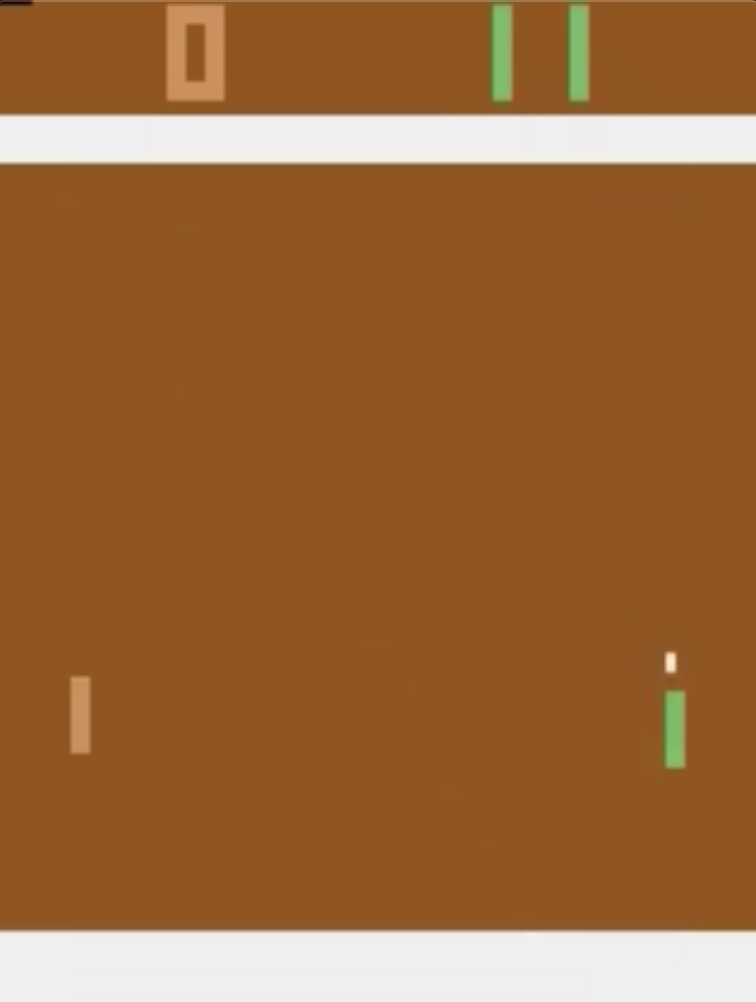
\includegraphics[width=00.95\textwidth]{Figures/single_env_cnn-lstm_agent.png}
        \caption{This is showing the fully PPO2 trained CNN-LSTM agent, under-the-hood transformed to work with a single environment, showcasing its superhuman abilities. Believe it or not, the agent actually returned the ball right after this step. Also note the score, 11-0, anecdotal confirmation of the agent's dominance and strong learning performance.}
        \label{fig: single_env_cnn-lstm_agent}
    \end{subfigure}
    \begin{subfigure}[t]{0.48\linewidth}
        \captionsetup{width=0.95\linewidth}
        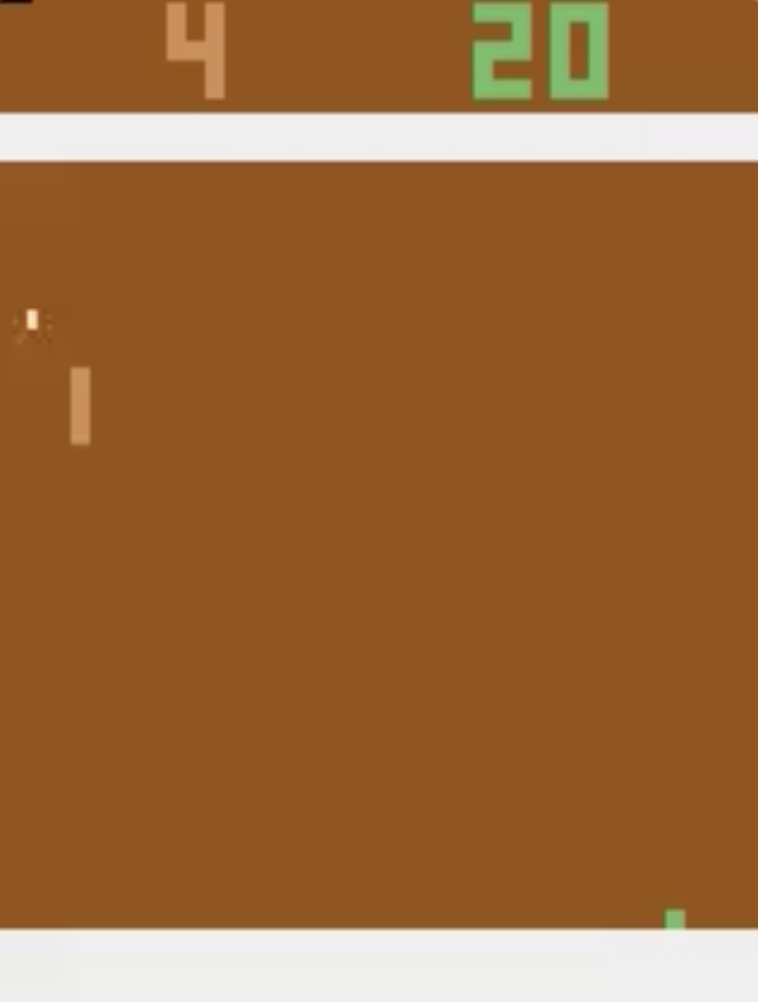
\includegraphics[width=0.95\textwidth]{Figures/single_env_mmn_agent.png}
        \caption{This is showing the fully "trained" MMN agent. Both the observation feature QBN and hidden state QBN have been fully trained, as in Figures \ref{fig: obs_qbn_loss} \& \ref{fig: hid_state_qbn_loss} respectively, and inserted into the original CNN-LSTM policy network as shown in Figure \ref{fig: net_architecture_overview}. Here, the MMN agent winning the game, but it obvious that it lost a little bit of performance compared to the original policy (look at the score). Also, if you check the \href{https://github.com/nicholasRenninger/NeuralMooreMachine_Experiments}{github repo} to see gifs of the MMN agent, where it is certainly clear that while still performant, the quantization has made it appear visually less "smooth".}
        \label{fig: single_env_mmn_agent}
    \end{subfigure}
    \caption{Visualizations of the CNN-LSTM and MMN Pong Agents in Different Environments}
    \label{fig: environments}
\end{figure*}